% !TEX root = diss.tex

\chapter{The Relationship Between Arrhenius Pre-factors with Non-Covalent Binding}
\label{ch:arrhenius}

\section{Introduction}


DiLabio and Ingold\cite{DiLabio2005} previously investigated the formal HAT reaction of the iminoxyl/oxime self-exchange reaction. In that paper, they compiled a table of parameters from the phenomenological Arrhenius equation for a series of interesting reactions, which appear here in~\ref{tab:Arrhenius-expt}.\cite{Kreilick1966, Mader2004, Mahoney1970, DaRooge1967, Howard1973, Foti1994, Chenier1974, Chenier1975} These are thermoneutral self-exchange reactions of oxygen-centred $\pi$-radicals,\footnotemark\ and other nearly thermoneutral reactions involving the destruction and formation of oxygen-centred $\pi$-radicals, reactions 3.1 and 3.2, respectively:

\begin{align}
  \ch{$\pi$-RO^. + ROH &-> ROH + $\pi$-RO^.} \hspace{2cm} \Delta H = 0 \\
  \ch{$\pi$-R}^\prime\ch{O^. + ROH &-> R}^\prime\ch{OH + $\pi$-RO^.} \hspace{2cm} \Delta H \approx 0
\end{align}

\newcommand{\tabFig}[2][0.35]{\includegraphics[scale=#1]{figures/#2.eps}}

\begin{table}[!ht]
  \footnotesize
  \centering
  \caption[Table of results for (nearly) thermoneutral reactions studied.]{Table of results for (nearly) thermoneutral reactions studied. Units for $\Delta H$, $E_a$, and calculated binding energy (BE) are \kcalmol, and $\log A$ and $k$ are \Ms.\ References to the original literature are included with the Complex ID number. $^\dagger$Calculated binding energies involve non-minimum structure containing one or more small imaginary frequencies. Adapted with permission from Reference \protect\citenum{DiLabio2005}. Copyright (2005) American Chemical Society.}
\begin{tabular}{l >{\centering}m{1.5cm} >{\centering}m{1.5cm} >{\centering}m{1.2cm} >{\centering}m{1.2cm} >{\centering}m{1.2cm} >{\centering}m{1.2cm} >{\centering}m{0.8cm} m{0em}}
  ID & \ch{RO^.}/\ch{R}$^\prime$\ch{O^.} & \ch{ROH} & $\Delta H$ & $\log~A$ & $E_a$ & $k$ & BE & \\
  \toprule
  1\cite{Kreilick1966} & \tabFig{3tBuPhO} & \tabFig{3tBuPhOH} & 0.0 & 3.7 & 1.2 & 3.3\E{2} & -10.8 &\\
  2\cite{Mader2004} & \tabFig{4MeC5H4ONO} & \tabFig{4MeC5H6NOH} & -2.0 & 3.8 & 3.8 & 10 & -14.8 &\\
  3\cite{Kreilick1966}$^\dagger$ & \tabFig[0.4]{2tBuNO} & \tabFig[0.4]{2tBuNOH} & 0.0 & 5.1 & 3.5 & 3.3\E{2} & -10.1 &\\
  4\cite{Mahoney1970,DaRooge1967}$^\dagger$ & \tabFig{3tBuPhO} & \tabFig{tBuPhOH} & 4.2 & 5.5 & 4.8 & 93 & -10.0 &\\
  5\cite{Howard1973} & \tabFig[0.7]{tBuOO} & \tabFig{3tBuPhOH} & -7.0 & 4.2 & 0.5 & 7\E{3} & -6.8 &\\
  6\cite{Kreilick1966}$^\dagger$ & \tabFig[0.7]{Ph2NO} & \tabFig[0.7]{Ph2NOH} & 0.0 & $>$7 & - & $>$10$^7$ & -13.6 &\\
  7\cite{Foti1994} & \tabFig{PhO} & \tabFig{2hydroxynaphthalene} & -2.2 & 8.3 & 2.3 & 4\E{6} & -8.6 &\\
  8\cite{Chenier1974}$^\dagger$ & \tabFig[0.7]{tBuOO} & \tabFig{PhOH} & 0.3 & 7.2 & 5.2 & 3\E{3} & -5.5 &\\
  9\cite{Chenier1974}$^\dagger$ & \tabFig[0.7]{tBuOO} & \tabFig{2hydroxynaphthalene} & -1.9 & 6.4 & 2.6 & 3\E{4} & -5.6 &\\
  10\cite{Chenier1975}$^\dagger$ & \tabFig[0.7]{tBuOO} & \tabFig{alphatetralinperoxide} & 1.4 & 6.0 & 4.5 & 7\E{2} & -8.0 &
\end{tabular}
\label{tab:Arrhenius-expt}
\end{table}

\footnotetext{\noindent A $\pi$-radical is one in which the SOMO is orthogonal to the plane of the molecular framework, i.e.\ of $\pi$-symmetry. Note that free alkoxyl radicals cannot be distinguished as either $\sigma$ or $\pi$-radicals, as the SOMO is degenerate, or free to rotate with respect to the rest of the molecular framework. Therefore, only the geometry of the radical-molecule complex can resolve the symmetry of the SOMO.}

Although it is well known that reactions of this nature involve remarkably low activation energies ($E_a$),\cite{Lucarini1996, Mahoney1970a, Mahoney1975, Korcek1972} they also have unusually low Arrhenius pre-exponential factors ($A$), or as they shall be referred to herein, \emph{A-factors}. As a result, these reactions are generally slower than expected, evidence for which is summarized in~\ref{tab:Arrhenius-expt}: The measured A-factors are small, and range from $10^{3.5}$--$10^{8.3}$ \Ms.\
In the past, this has been attributed to steric shielding around the oxygen atoms, resulting in a large entropic barrier.\cite{DiLabio2005} Importantly, it was noted that the degree of steric shielding on the oxygen atom appears to play an important role in the order of the A-factor; systems with greater bulk have lower A-factors, while non-shielded systems have larger A-factors.

Stereo-electronic effects are known to play an important role in HAT, and have been studied extensively.\cite{Finn2004, Salamone2011, Pischel2001, Griller1981, Bietti2011, Salamone2012, Malatesta1982, Salamone2014} Although the abstraction of a specific hydrogen atom may be more thermodynamically favourable than others on a given substrate, if it is not accessible due to steric constraints, abstraction will not occur at this site. Otherwise, additional steric bulk can lead to significant reductions in reactivity, through destabilization of the TS complex, or by forcing additional processes involving conformational changes in order to reach the appropriate TS structure. For example, in reactions of tertiary acetamides with \cumo,\cite{Salamone2014} where abstraction occurs mainly from C-H bonds $\alpha$ to the nitrogen atom, a two-fold decrease in the rate constant (normalized for the number of equivalent hydrogen atoms) is observed in going from $N,N$-dimethylacetamide to $N,N$-diisobutylacetamide ($k_H$ = $2.0 \times 10^5$ and $7.8 \times 10^4$ \Ms, respectively). The decrease in rate constant is attributed to the steric clash between the methyl groups of \cumo\ and the isobutyl groups of $N,N$-diisobutylacetamide.

Upon first inspection, all of the reactions in~\ref{tab:Arrhenius-expt} appear to be of a similar nature. Each reaction involves the breaking and formation of O-H bonds as the thermodynamic driving force. All of these bonds are expected to be of comparable strength, therefore, differences should not contribute significantly to reaction barriers in a Bell-Evans-Polanyi principle fashion. Hence, the large degree of variance in their rate constants ($k$) is somewhat surprising. These reactions are closely related to the self-exchange reaction between phenol and phenoxyl,\cite{Mayer2002} in which a strong molecule-radical pre-reaction complex is formed, ca. 10 \kcalmol\ below the separated reactants. It is therefore expected that most, if not all, of the systems in~\ref{tab:Arrhenius-expt} should exhibit a similar molecule-radical complex; granted, the strength of the interaction will vary because of steric repulsion.

Currently, there has been no comprehensive investigation of the relationship between the pre-reaction complex and the kinetics of a reaction. Using the reactions and data in~\ref{tab:Arrhenius-expt}, we ask the question: \emph{Do A-factors have a correlation with non-covalent binding energies of the pre-reaction complex?} This is a reasonable question as non-covalent binding and steric hinderance represent a loss of degrees of freedom and therefore entropy,\footnotemark\ which ultimately determines the A-factor magnitude. If the answer to the question is yes, then non-covalent binding may be useful as a diagnostic for the ``looseness'' or ``tightness'' of a TS complex, in addition to providing an important link between theory and experiment.

\footnotetext{Recall from Equation~\ref{eq:afactor} that the A-factor can be related to TST such that the primary variable is entropy ($\Delta^\ddagger S^0$).}

\section{Computational methods and details}

Density-functional theory (DFT) calculations were carried out using the Gaussian-09 software package.\cite{Frisch2009} Care was taken to obtain minimum energy structures through detailed conformational analysis. For this, the BLYP density-functional\cite{Becke1988,Lee1988} was utilized, paired with the empirical D3 dispersion correction\cite{Grimme2010} with the recommended Becke-Johnson damping functions,\cite{Johnson2006} as well as our groups' own basis set incompletion potentials (BSIPs),$^*$\jnote{update citation} and minimal MINIs basis sets.\cite{Huzinaga1984} The use of minimal basis sets corrected for basis set incompleteness allows DFT-based methods (as opposed to semi-empirical or force-field based approaches) to be used efficiently in performing a large number of calculations. Minimum energy conformers of the monomers (substrates and radicals) were first obtained by manual manipulation of the necessary dihedral bond angles, followed by geometry optimization and vibrational analysis.

The lowest energy radicals and substrates were combined to generate the appropriate pre-reaction complexes. These pre-reaction complexes were subject to conformational analysis using the same BLYP-D3(BJ)-BSIP/MINIs method. Geometries were initially manipulated by hand. It became apparent that manual manipulation resulted in an unsatisfactory exploration of the conformational space. To solve this, all the necessary dihedral angles were scanned systematically using a combination of scripts.\bibnote{The Escher program\cite{escher} was used to generate a Z-matrix with specific dihedral angles. This geometry was then systematically scanned using simple shell scripts.} All manipulated geometries were subject to optimization. For each complex, the top 5--10 complex geometries were subject to further optimization using a higher level of theory (BLYP-D3(BJ)-BSIP/pc-1) to obtain the final minimum energy pre-reaction complex structures. Due to the free rotation of groups such as $t$-butyl and methyl, some of the optimized pre-reaction complex structures contain small imaginary frequencies, and thus do not represent proper stationary states. Several measures were taken to resolve this, however, no resolution was obtained in many cases. Regardless, the complexes adequately represent the pre-reaction complex and differences in ``true'' binding energies can likely be ignored.

To obtain accurate pre-reaction complex binding energies, the substrates and complexes were subject to single-point energy calculations using the LC-$\omega$PBE long-range corrected density functional\cite{Vydrov2006,Vydrov2006a} with D3(BJ) dispersion corrections and pc-2 basis sets with truncated $f$-type functions (pc-2-spd).\cite{Johnson2013} This method was selected on the recommendation of work by \citet{Johnson2013}, which demonstrated the accuracy of this method for the calculation of NCIs. On the basis of the reported mean absolute error in Reference \citenum{Johnson2013} for the S66 benchmark set of sixty-six different non-covalently interacting dimers,\cite{Rezac2011} the calculated binding energies reported herein from the LC-$\omega$PBE-D3(BJ)/pc-2-spd level of theory carry an estimated 0.2 \kcalmol\ margin of error.

\section{Results and discussion}

The theoretically determined electronic binding energies calculated for the lowest energy pre-reaction complex of each system are listed in~\ref{tab:Arrhenius-expt}. The logarithm of A-factor against binding energy was plotted, as shown in~\ref{fig:Arrhenius}. The overall correlation is quite poor ($R^2$ = 0.33), however much of the data is grouped about a single, well correlated line ($R^2$ = 0.95). The intercept of the fitted line which corresponds to zero binding energy is 8.63, a value which is in line with what has been cited as the expected A-factor for HAT reactions, \emph{viz. }$10^{8.5\pm0.5}$ \Ms.\cite{Benson1976} These results suggest that the observed correlation is genuine, that is, NCIs may have an impact on A-factors. I shall demonstrate that the data which do not correlate are reasonable outliers. In fact, using simple rationale I shall demonstrate that different regimes of steric bulk results in different processes leading to the TS complex. As a result, deviations from the relationship between A-factor and binding energy are observed.

\begin{figure}[!htbp]
  \centering
  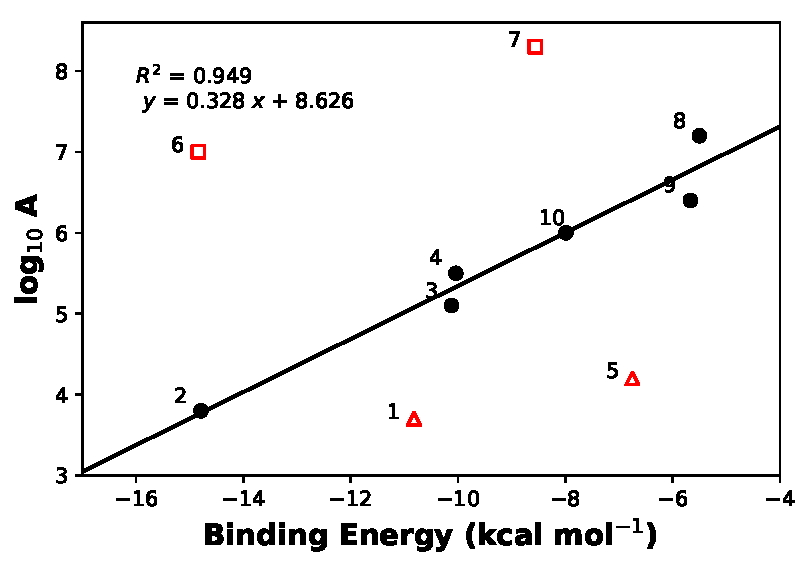
\includegraphics[width=0.85\textwidth]{figures/arrhenius-scatter.pdf}
  \caption[Plot of logarithm of A-factor against binding energy.]{Plot of logarithm of A-factor against binding energy. Only the black points were included in the line fitting (slope = 0.328 \kcalmol, intercept = 8.626 \kcalmol, and $R^2$ = 0.949). Red points with open faced markers indicate outliers, \emph{vide infra}. The inclusion of complexes 1, 5, and 7 result in an $R^2$=0.334. Complex 6 is always omitted from line fitting as the experimental A-factor is approximate.}
\label{fig:Arrhenius}
\end{figure}

In order to illustrate this, consider the fundamental properties of the HAT reactions involved herein. There are two important concerted reaction mechanisms that are possible, namely direct HAT or PCET.\@ Specifically, we must consider the geometric constraints in which these reaction mechanisms occur. For direct HAT to occur, the SOMO of the radical must overlap with the O-H $\sigma^*$ anti-bonding orbital. This may require the rotation of the hydrogen atom donating hydroxyl group out of the plane. The rotation of a phenolic hydroxyl group has an energy barrier that follows a $\cos^2 \theta$ relationship, and can be as high as 3.1 \kcalmol\ on the basis of the rotational barrier in phenol.\cite{Kim1994} For a PCET mechanism to occur, there are two possible geometries: Either the SOMO of the radical overlaps can overlap with the corresponding oxygen lone pair $p$-orbital, as seen in the work of \citet{Mayer2002}; or a lone pair-$\pi$ or $\pi$-$\pi$ bonding overlap between the radical and substrate can occur, as seen in the work of \citet{DiLabio2007}. Due to time constraints, I did not seek to obtain TS complex structures. Nonetheless, from the pre-reaction complex one can surmise the most likely TS complex. Thus, by applying these basic principles, it is possible to rationalize deviations from the trend observed in~\ref{fig:Arrhenius}.

\begin{figure}[!htbp]
\centering
\hspace*{-1.8cm}
\begin{minipage}{8cm}
  \centering
  \begin{overpic}[width=\textwidth]{figures/complex2_hbond}
  \put(5,91) {\large\textbf{A.}}
\end{overpic}
\end{minipage}%
\begin{minipage}{8cm}
  \centering
  \begin{overpic}[width=\textwidth]{figures/complex3_hbond}
  \put(5,90) {\large\textbf{B.}}
\end{overpic}
\end{minipage}
\caption[Three-dimensional structures of pre-reaction complexes 2 (TEMPO-H and 4-oxo-TEMPO) and 3 (di-$t$-butyl-hydroxylamine and di-$t$-butyl-nitroxyl).]{Three-dimensional structures of \textbf{A} complex 2, and \textbf{B} complex 3. Hydrogen bond distances are shown in units of \AA.\@ The elements are coloured as white for carbon, light blue for hydrogen, red for oxygen, and blue for nitrogen.}
\label{fig:com2-3}
\end{figure}

We shall begin by examining the points which fall on the expected line, complexes 2--4 and 8--10. The examination of all these pre-reaction complexes reveals that an additional process that has a moderate energetic barrier is required in order for formal HAT reactions to proceed. Complexes 2 and 3 are shown in~\ref{fig:com2-3}, and are very similar in structure. Both are hydroxylamine-nitroxyl couples with similar degrees of steric bulk adjacent to the reacting centres. The $t$-butyl groups of 3, and the methyl groups of 2 prevent the alignment of the NO-H-ON frameworks in a PCET manner. In order to reach the TS complex, both 2 and 3 must bring methyl groups within close proximity for direct HAT to occur. In the most stable stacked conformation, complex 4, as seen in~\ref{fig:com4}, cannot undergo PCET as the steric clash of the para-position $t$-butyl groups prevent $\pi$-$\pi$ overlap. In order to react via direct HAT, the hydroxyl group must rotate further out of the aromatic plane, or the bulky para-position $t$-butyl groups must come into close proximity. Alternatively, an open conformation for complex 4 is possible, which lies ca. 2 \kcalmol\ higher in energy than the stacked complex, a result which is also consistent with the observed trend-line. From the open conformation, PCET is still not possible due to the steric bulk of the ortho-position $t$-butyl groups of the radical, thus this reaction likely proceeds through a direct HAT mechanism.

\begin{figure}[!htbp]
\centering
\hspace*{-1.8cm}
\begin{minipage}{8cm}
  \centering
  \begin{overpic}[width=\textwidth]{figures/complex4_hbond}
  \put(10,100) {\large\textbf{A.}}
\end{overpic}
\end{minipage}%
\begin{minipage}{8cm}
  \centering
  \begin{overpic}[width=\textwidth]{figures/complex4_steric}
  \put(0,100) {\large\textbf{B.}}
\end{overpic}
\end{minipage}
\caption[Three-dimensional structure of pre-reaction complex 4 between 2,4,6-tri-$t$-butylphenol and  4-$t$-butylphenoxyl.]{Three-dimensional structure of pre-reaction complex 4 between 2,4,6-tri-$t$-butylphenol and  4-$t$-butylphenoxyl. \textbf{A} demonstrates the hydrogen bond distances in units of \AA, and the out-of-plane rotation by 35.2$^\circ$ of the phenolic hydroxyl group. \textbf{B} demonstrates the steric clash (highlighted by red box) between the para-position $t$-butyl groups. The elements are coloured as white for carbon, light blue for hydrogen, and red for oxygen.}
\label{fig:com4}
\end{figure}

Complexes 8 and 9 are similar systems, in which \ch{$t$-BuOO^.} reacts with unhindered phenolic substrates. As seen by the structures in~\ref{fig:com8-9}, the bound complexes are somewhat dissimilar. The hydroxyl group of complex 8 is rotated out of the plane 24$^\circ$, while in complex 9 the hydroxyl group lies entirely in the plane. It is likely that the larger aromatic system of 2-naphthol results in a larger OH rotational barrier, and thus the most favourable conformation is entirely in the plane. Complex 8 was previously studied by \citet{DiLabio2007}, where it was demonstrated that a partial bonding interaction exists between the peroxyl lone-pair and phenolic $\pi$-system, and thus formal HAT proceeds through a PCET mechanism. Although the pre-reaction complexes are somewhat dissimilar, the conformational changes necessary to reach a PCET TS complex, similar to that reported in reference \citenum{DiLabio2007}, are likely not dramatically different in terms of energetic barriers. Any small differences result in noise in the observed trend.

\begin{figure}[!htbp]
\centering
\hspace*{-1.8cm}
\begin{minipage}{8cm}
  \centering
  \begin{overpic}[width=\textwidth]{figures/complex8_hbond}
  \put(0,110) {\large\textbf{A.}}
\end{overpic}
\end{minipage}%
\begin{minipage}{8cm}
  \centering
  \begin{overpic}[width=\textwidth]{figures/complex9_hbond}
  \put(0,100) {\large\textbf{B.}}
\end{overpic}
\end{minipage}
\caption[Three-dimensional structures of pre-reaction complexes 8 ($t$-butylperoxyl and phenol) and 9 ($t$-butylperoxyl and 2-naphthol).]{Three-dimensional structures of pre-reaction complexes \textbf{A.} 8 ($t$-butylperoxyl and phenol) and \textbf{B.} 9 ($t$-butylperoxyl and 2-naphthol). Hydrogen bond distances are shown in units of \AA.\@ Complex 8 has an out of plane rotation of the phenolic hydroxyl group of 24.1$^\circ$. The elements are coloured as white for carbon, light blue for hydrogen, and red for oxygen.}
\label{fig:com8-9}
\end{figure}

Complex 10 is unique in that it is the only reaction between a peroxide and a peroxyl radical. The self-exchange reaction between \ch{HOO^.} and \ch{HOOH} can be considered the simplest reference for the reaction of $\alpha$-tetralin peroxide with $t$-butylperoxyl. To the best of my knowledge, the mechanism of the hydroperoxyl-hydrogen peroxide couple has not been characterized as either PCET or direct HAT previously in the literature, although the TS structure has been previously reported.\cite{Isborn2005} Using this structure, calculations reveal a lone pair-lone pair interaction leading to partial bonding in the TS, i.e.\ a PCET mechanism. (See Appendix~\ref{ap:arrhenius},~\ref{fig:hooh-ooh}). Also the hydroperoxyl-hydrogen peroxide couple appears to prefer an \ch{H-O-O-H} dihedral angle of 90$^\circ$, so that the two non-reacting hydrogen atoms oriented 180$^\circ$ away from one another. Orienting substituents directly away from one another is likely the most stable TS structure for all peroxyl-peroxide formal HAT reactions. In order for complex 10 to achieve a similar TS structure, $t$-butylperoxyl and $\alpha$-tetralin peroxide must reorganize to avoid steric clash, likely through a rotation of the \ch{HOO} moiety of $\alpha$-tetralin peroxide.

\begin{figure}[!htbp]
\centering
\hspace*{-1.8cm}
\begin{minipage}{8cm}
  \centering
  \begin{overpic}[width=\textwidth]{figures/complex10_hbond}
  \put(0,100) {\large\textbf{A.}}
\end{overpic}
\end{minipage}%
\begin{minipage}{8cm}
  \centering
  \begin{overpic}[width=\textwidth]{figures/complex10_steric}
  \put(0,100) {\large\textbf{B.}}
\end{overpic}
\end{minipage}
\caption[Three-dimensional structure of pre-reaction complex 10 between $t$-butylperoxyl and $\alpha$-tetralin peroxide.]{Three-dimensional structure of pre-reaction complex 10 between $t$-butylperoxyl and $\alpha$-tetralin peroxide. \textbf{A} demonstrates the hydrogen bond distances in units of \AA. \textbf{B} demonstrates the incorrect orientation of the peroxyl-peroxide units for a PCET TS complex to occur. The elements are coloured as white for carbon, light blue for hydrogen, and red for oxygen.}
\label{fig:com10}
\end{figure}

Once again, complexes 2--4 and 9--10 follow the observed trend. In all cases, these complexes must undergo an additional conformational change with a small energy barrier in order to reach the pre-reaction complex which leads directly to the TS complex. This is illustrated in~\ref{fig:afactor-trend},

\begin{figure}[!htbp]
  \centering
  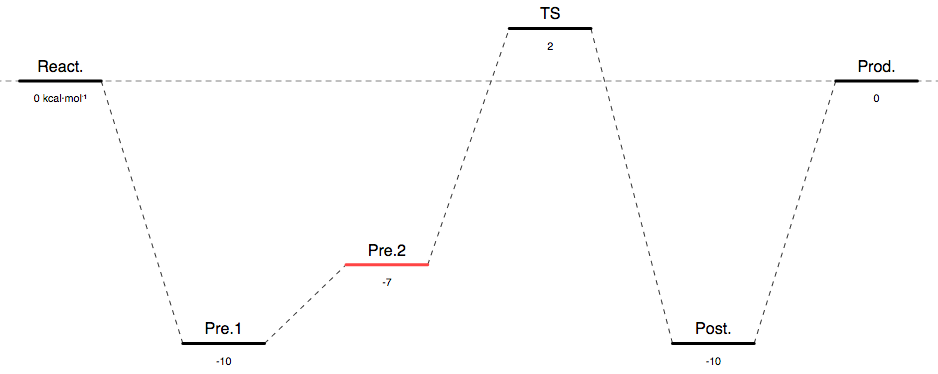
\includegraphics[width=\textwidth]{figures/afactor-trend.png}
  \caption[Reaction coordinate illustrating a conformational change to a second pre-reaction complex prior to transition state formation.]{Reaction coordinate illustrating a conformational change to a second pre-reaction complex prior to transition state formation. Energies are estimated for a self-exchange reaction. React. = reactants, Pre.1 = lowest energy pre-reaction complex, Pre.2 = postulated higher energy pre-reaction complex involving conformational change, TS = transition state, Post. = post-reaction complex, Prod. = products.}
\label{fig:afactor-trend}
\end{figure}

Consider next the points which sit above the trendline, complexes 6 and 7. The A-factor for complex 6 is approximate and thus does not get factored into the line fitting. In both cases, the non-covalently bound complexes are in a slipped-parallel $\pi$-stacked conformation. Complex 7 in particular is very similar to the phenol-phenoxyl couple, except with 2-naphthol instead of phenol. Therefore, it is possible to infer that both of these reactions take place through a PCET mechanism. In fact, these pre-reaction complexes are optimally aligned to achieve the appropriate TS complexes. Therefore, in contrast to the observed trend, complexes 6 and 7 do not require an additional conformational change to approach the TS complexes, as illustrated in~\ref{fig:afactor-direct}.

\begin{figure}[!htbp]
  \centering
  
\includegraphics[width=\textwidth]{figures/afactor-direct.png}
  \caption[Reaction coordinate illustrating no conformational change before moving from pre-reaction complex to the transition state.]{Reaction coordinate illustrating no conformational change before moving from pre-reaction complex to the transition state. Energies are estimated based on a self-exchange reaction. React. = reactants, Pre. = lowest energy pre-reaction complex, TS = transition state, Post. = post-reaction complex, Prod. = products.}
\label{fig:afactor-direct}
\end{figure}

Lastly, consider the points which fall below the trendline, complexes 1 and 5. In both cases, a high degree of steric repulsion likely does not allow for a PCET mechanism. Complex 1 is the self-exchange reaction between the very bulky 2,4,6-tri-$t$-butylphenol-2,4,6-tri-$t$-butylphenoxyl couple, as seen in~\ref{fig:com1-5} A. As a result of steric shielding around the reaction centres, the most stable pre-reaction complex is stacked to maximize dispersion interactions, but does not have a hydrogen bond, which is unique among the ten reaction couples studied herein. Therefore, these must be a higher-energy hydrogen-bonded pre-reaction couple that leads to the HAT transfer. Note however, that there is a barrier to rotation of the hydroxyl group to 90$^\circ$ out of the plane for direct HAT to occur.

\begin{figure}[!htbp]
\centering
\hspace*{-1.8cm}
\begin{minipage}{8cm}
  \centering
  \begin{overpic}[width=\textwidth]{figures/complex1}
  \put(0,100) {\large\textbf{A.}}
\end{overpic}
\end{minipage}%
\begin{minipage}{8cm}
  \centering
  \begin{overpic}[width=\textwidth]{figures/complex5}
  \put(0,100) {\large\textbf{B.}}
\end{overpic}
\end{minipage}
\caption[Three-dimensional structures of pre-reaction complexes 1 (2,4,6-tri-$t$-butylphenoxl and 2,4,6-tri-$t$-butylphenoxyl) and 5 (2,4,6-tri-$t$-butylphenol and $t$-butylperoxyl).]{Three-dimensional structures of pre-reaction complexes \textbf{A.} 1 (2,4,6-tri-$t$-butylphenoxl and 2,4,6-tri-$t$-butylphenoxyl) and \textbf{B.} 5 (2,4,6-tri-$t$-butylphenol and $t$-butylperoxyl. Distances in unit of \AA and angles are shown in degrees. The elements are coloured as white for carbon, light blue for hydrogen, and red for oxygen.}
\label{fig:com1-5}
\end{figure}

Complex 5 is the 2,4,6-tri-$t$-butylphenol-$t$-butylperoxyl reaction couple. The lowest-energy pre-reaction complex contains a hydrogen bond, however the hydroxyl group is rotated 90$^\circ$ out of the plane. It is likely that as with complex 1, a pre-reaction complex without a hydrogen bond forms first. However, in complex 1 there is less steric clashing, thus the formation of a hydrogen bond is favourable. There is a barrier to rotation\footnotemark\ of the hydroxyl group that is about 4.1 \kcalmol. Note the unusual character of the hydrogen bond formed. Optimal hydrogen bonds are nearly linear so that there is both a dipole-dipole interaction and an orbital interaction such that the lone pair of the acceptor donates electron density into the OH $\sigma^*$ anti-bonding orbital.\cite{Jeffrey1997} In the case of complex 5, the hydrogen bond is nearly perpendicular, resulting in only an orbital interaction.\footnotemark\ The lowest energy pre-reaction complex 5 is comparable to that of complex 8, the TS of which as published in reference \citenum{DiLabio2007}. Formal HAT in complex 8 takes place through a PCET mechanism, however due to steric shielding it is unlikely that the correct $\pi-\pi$ orbital overlap can occur for PCET to occur. Therefore, this reaction can also be described as taking place through a direct HAT mechanism.

\footnotetext{Calculated as the difference in energy between the in-plane and out-of-plane structures of 2,4,6-tri-$t$-butylphenol at the LC-$\omega$PBE-D3/6-311+G(2d,2p) level of theory.}

\footnotetext{The hydrogen bonding nature of this interaction has been verified using the NCIplot software.\cite{Johnson2010,ContrerasGarcia2011} These results can be found in Appendix~\ref{ap:arrhenius},~\ref{fig:nciplot}.}

Complexes 1 and 5 fall below the trendline of $\log A$ vs calculated binding energy. Because of the steric bulk of 2,4,5-tri-$t$-butylphenol, the hydroxyl group must rotate $90^\circ$ out of plane from the minimum energy structure,  in order for HAT to occur. This process has an energy barrier of about 4.1 \kcalmol. For complex 1, this results in a higher energy pre-reaction complex, while for complex 5 this results in a lower energy pre-reaction complex. However, because the formation of a non-hydrogen bonded complex must necessarily come first, the experimental A-factor does not correlate with the calculated binding energy as observed for complexes 2--4 and 8--10, which undergo a conformational change with little or no barrier. That is to say, the rotation of the phenol hydroxyl group is an additional process with a significant energy barrier, and thus explains the difference in trends.

\section{Summary}

In this investigation, I report the lowest energy pre-reaction complexes for a series of thermoneutral or nearly thermoneutral HAT reactions. I have plotted the theoretically determined electronic binding energies against the logarithm of experimentally determined A-factors. These results demonstrate that the A-factor is correlated to some extent with the binding energy, given that the reactions proceed through energetically similar pathways. The results herein can be sorted into three bins:

\begin{enumerate}
  \item Complexes which require a small conformational with no barrier to approach the TS structure fall onto the observed trendline. This appears to be the most likely case for formal HAT reactions.

  \item Complexes which are optimally aligned to approach the TS structure. This was the case for complexes 6 and 7.

  \item Complexes which the full $90^\circ$ rotation of the phenolic hydroxyl group is required for formal HAT to occur. This is the case when the phenol is highly sterically shielded.
\end{enumerate}

These results indicate that different regimes of steric interactions lead to different chemical processes in seemingly similar reactions. As a results, non-covalent binding can be used as a metric for kinetics parameters, however, it cannot full describe the entropic factors which contribute to the A-factor. One must first determine the relationship between the pre-reaction and TS complex.

Additional work is necessary to extend these results. In particular, a larger sample of data points should be used. Regardless, the results herein represent a novel attempt to link theory and experiment. Given that obtaining the full PES for large molecules is currently computationally impractical, these results serve as a seed for developing a fundamental understanding of complex formal HAT reactions.
